PIPE (Platform Independent Petri Net Editor) è un software progettato per supportare la modellazione, l'analisi e la simulazione delle reti di Petri. Si tratta di uno strumento potente e versatile che offre un'interfaccia intuitiva per rappresentare visivamente sistemi complessi attraverso diagrammi basati sulle reti di Petri. PIPE si distingue per la sua capacità di combinare un approccio grafico user-friendly con strumenti avanzati di analisi e simulazione, rendendolo una scelta ideale per ingegneri, ricercatori e sviluppatori che lavorano su sistemi distribuiti, processi aziendali e reti di comunicazione.

\begin{figure}
    \centering
    \begin{minipage}[b]{.45\textwidth}
        \centering
        
\includegraphics[width=\textwidth]{figure/pipe/pipe_logo.png}
        \caption{Logo di PIPE 2}
        \label{fig:pipe_logo}
    \end{minipage}
    \hfill
    \begin{minipage}[b]{.45\textwidth}
        \centering
        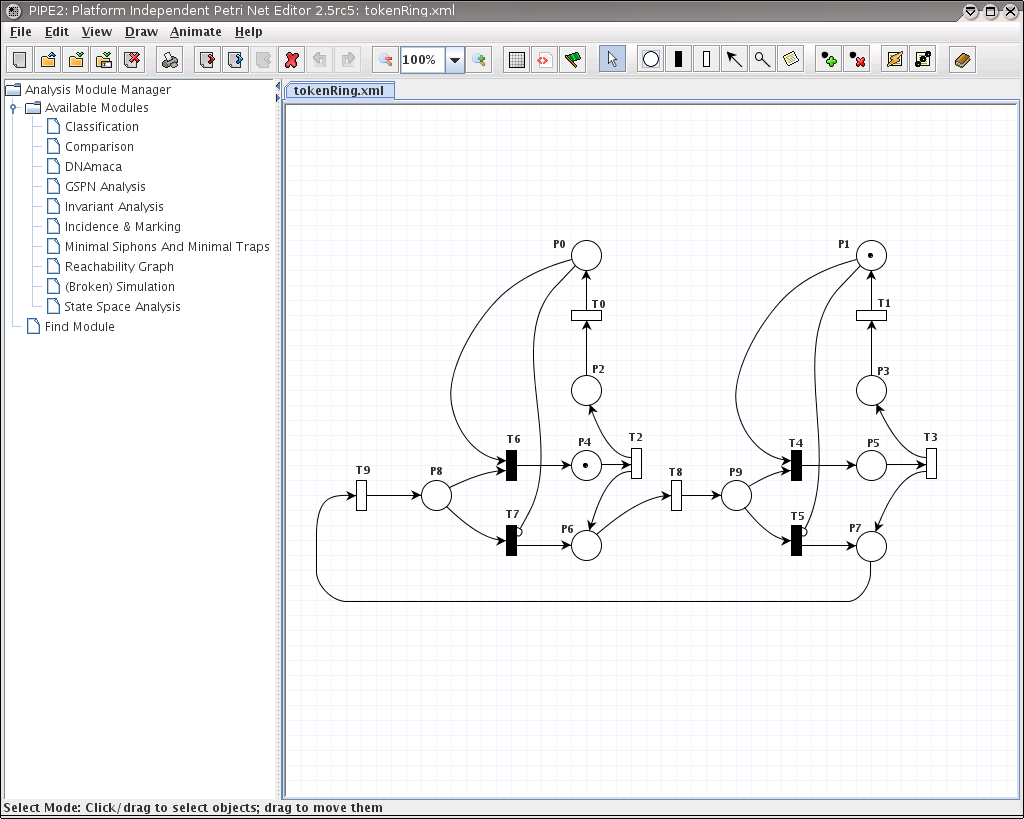
\includegraphics[width=\textwidth]{figure/pipe/pipe_example.png}
        \caption{Esempio di PIPE 2}
        \label{fig:pipe_example}
    \end{minipage}
\end{figure}

\newpage
Segue ora un breve elenco riportante alcune funzionalità di PIPE 2 che ne hanno portato alla scelta come software per la realizzazione di questo progetto.

\begin{itemize}
    \item \textbf{Interfaccia grafica intuitiva}
    PIPE offre un ambiente visuale semplice ma potente che consente agli utenti di progettare reti di Petri in modo interattivo. Gli elementi principali del modello, come posti (posti di memoria o risorse, rappresentati da cerchi), transizioni (eventi o processi, rappresentati da rettangoli) e archi direzionali (che collegano posti e transizioni), possono essere creati e configurati facilmente con pochi clic. Questa semplicità d'uso riduce la curva di apprendimento per i principianti e accelera il lavoro degli esperti.
    
    \item \textbf{Progettazione di reti di Petri}
    Con PIPE è possibile costruire reti di Petri che rappresentano la logica e il flusso di informazioni di un sistema. Grazie al supporto per la modellazione grafica, l'utente può rappresentare visivamente il comportamento del sistema, rendendo più comprensibile la struttura complessiva. Ad esempio, un sistema produttivo può essere rappresentato da posti che indicano le risorse disponibili, transizioni che rappresentano i processi produttivi e archi che mostrano le relazioni tra risorse e processi.
    
    \item \textbf{Proprietà, attributi e personalizzazione}
    Uno degli aspetti distintivi di PIPE è la possibilità di aggiungere attributi dettagliati agli elementi della rete. Ogni arco, posto o transizione può essere personalizzato con proprietà specifiche, come i pesi degli archi, i tempi di ritardo associati alle transizioni o altre caratteristiche peculiari del sistema. Questo consente di creare modelli estremamente accurati, in grado di rappresentare fedelmente la complessità del sistema reale.
    
    \item \textbf{Analisi avanzata e simulazione dinamica}
    PIPE non si limita alla semplice creazione di reti di Petri, ma offre anche potenti strumenti di analisi e simulazione. L'utente può eseguire simulazioni per osservare il comportamento dinamico del sistema nel tempo, identificando colli di bottiglia, verificando proprietà di sicurezza (ad esempio, l'assenza di deadlock) o analizzando il throughput di risorse. Questo permette di testare le prestazioni del sistema in condizioni diverse e di ottenere preziose informazioni per ottimizzarne il design.
\end{itemize}